\section{Lighting}
\subsection{Interior Lighting}
Interior lighting follows a technology baseline approach, meaning that energy consumed by lighting is set by an assumed distribution of a particular lighting technology (e.g., T8 or linear LEDs), rather than following a lighting power density (LPD) allowance defined in a specific energy code version. The technology baseline approach recognizes that buildings typically do not use their full lighting power allowance. It also explicitly labels lighting technology and subsystems in the energy model for granular energy efficiency measure analysis.  

Two components specify interior lighting: the lighting power density and the interior lighting schedule.  The lighting power density is determined by the distribution of lighting technologies in the stock, the lighting technology properties, and the space type properties. The lighting schedule is determined by a default lighting schedule by space type, occupancy hour adjustments, and magnitude variability.

\subsubsection{Determining Lighting Power}
The technology baseline approach follows a similar process to how the ASHRAE 90.1 lighting subcommittee determines the LPD allowance for a given space type in ASHRAE 90.1. In the lighting subcommittee model (LSM), there are four kinds of lighting systems that together contribute to a target horizontal illuminance:

LPD = General Lighting + Task Lighting + Supplemental Lighting + Wall Wash Lighting \\

\begin{align}
\label{lsm_lpd_eqn}
LPD = \frac{\% LS_{1} \cdot fc}{RSDD \cdot TF_{1}} + \frac{\% LS_{2} \cdot fc}{RSDD \cdot TF_{2}} + \frac{\% LS_{3} \cdot fc}{RSDD \cdot TF_{3}} + \frac{\% LS_{4} \cdot fc}{RSDD \cdot TF_{4}}
\end{align}
where:\\
\begin{itemize}
\item \textbf{\%LS\textsubscript{i}} is the percent of the target horizontal illuminance value met by a specific lighting system\\
\item \textbf{fc} is the target horizontal illuminance value in lumens per ft\textsuperscript{2}\\
\item \textbf{RSDD} is room surface dirt depreciation, an estimate of how much surface dirt reduces light from reaching the horizontal plane\\
\item \textbf{TF\textsubscript{i}} is the total lighting factor, where TF = source luminous efficacy * coefficient of utilization * lighting loss factor (LFF)\\
\item \textbf{Source luminous efficacy} is the lighting technology efficacy in lumens per watt\\
\item \textbf{Coefficient of utilization} is a term that captures how much lighting from the luminaire reaches the horizontal plane\\
\item \textbf{LLF} is the lighting loss factor, where LLF  = luminaire dirt depreciation (LDD) * lamp lumen depreciation (LLD)\\
\end{itemize}

Values for all these terms are specified in the LSM.  The LSM is exact, using a specific lighting product, room geometry, distribution of lighting systems, and other properties to determine the lighting power density allowance for a given space type. ComStock differs from the LSM in several important ways. 

First, ComStock generalizes lighting technology (e.g., T8 linear fluorescent luminaires for general lighting) rather than modeling a specific lighting product.  Source efficacy, lighting loss properties, and radiant fractions are tied to lighting technology. Source efficacy values come from \cite{doe2015lmc} for older lighting technologies and \cite{doe2019ssl} for LEDs.  Radiant heat gain fractions come from \cite{ashrae_rp1282} for older lighting technologies and \cite{ashrae_rp1681} for LEDs.

Second, lighting technologies are broken out into lighting generations depending on the most common space lighting technology in that generation, as general lighting accounts for most ($\sim$80\%--90\%) of total lighting. High bay is treated as general lighting, and the lighting measure uses the general high bay technology for rooms with height $\ge$20 ft. Lighting generations 4--8 are all LED, with improving efficacy over time. Lighting generations and their technologies are detailed in Table \ref{tab:int_light_gens}, and lighting technology properties are detailed in Table~\ref{tab:int_light_techs_all}.

Third, the coefficient of utilization depends on both the luminaire properties and the room geometry, which complicates the calculation in the LSM. The ComStock model associates the coefficient of utilization entirely with room propertiesthat are independent of lighting technology.  ComStock further assumes that rooms of the same space type have similar enough properties that they can use the same coefficient of utilization. To retain some of the variation from the luminaire properties, each kind of lighting system has a different coefficient of utilization for each space type. 

Table~\ref{tab:int_light_space_types} in Appendix~\ref{appendix:a} details the target horizontal illuminance value, the fraction of the target illuminance met by the kind of lighting system, and the lighting system coefficient of utilization for each lighting space type. Lighting space types are defined in 90.1 and are determined based on a mapping of openstudio-standards space types to prototype lighting space types.

Fourth, the LSM assumes a high fraction of non-general lighting systems for certain space types. For example, half of the illuminance in retail sales spaces is from supplemental and wall wash lighting systems. In older lighting generations, there is a significant difference in source efficacy between general and non-general lighting systems. In lighting generation 2, general lighting assumes T8 linear fluorescent lamps at 94 lumens per watt, and supplemental and wall wash lighting assume halogens at 15 lumens per watt.  For retail spaces using the LSM values, that means half the lighting comes from lighting technologies roughly 6 times less efficient than the general lighting technology.  Although this may be appropriate for setting a code lighting allowance, most retail spaces meet a much greater percentage of their illuminance from more efficient general lighting technologies.  ComStock adjusts the lighting system fractions for commonly used space types so that around 80\%--90\% of lighting comes from the general lighting system. These changes are reflected in Table~\ref{tab:int_light_space_types} in Appendix \ref{appendix:a}.

Lastly, the LSM offers a generous allowance for lighting power density to account for the lighting loss factor over time. Including lighting losses and depreciation can result in a lighting power density ~40\% higher than when these terms are ignored. This resulted in unreasonably high installed lighting power densities; thus, ComStock assumes that most existing lighting systems were not designed to account for depreciation over time, and therefore excludes lighting loss and depreciation terms from the lighting power calculation.

With these changes, the LPD calculation simplifies to:
\begin{align}
\label{comstock_lpd_eqn}
LPD = \frac{\% LS_{1} \cdot fc}{\text{efficacy} \cdot CU_{1}} + \frac{\% LS_{2} \cdot fc}{\text{efficacy} \cdot CU_{2}} + \frac{\% LS_{3} \cdot fc}{\text{efficacy} \cdot CU_{3}} + \frac{\% LS_{4} \cdot fc}{\text{efficacy} \cdot CU_{4}}
\end{align}

where:\\
\begin{itemize}
\item \textbf{\%LS\textsubscript{i}} is the percent of the target horizontal illuminance value met by a specific lighting system\\
\item \textbf{fc} is the target horizontal illuminance value in lumens per ft\textsuperscript{2}\\
\item \textbf{Efficacy} is the source luminous efficacy of the lighting technology in lumens per watt\\
\item \textbf{CU} is the coefficient of utilization, a term that captures how much lighting from the luminaire reaches the horizontal plane.\\
\end{itemize}

The resulting LPDs are shown in Figure~\ref{fig:interior_lighting_lpd}.

\begin{table}
\small
\centering
\caption[Interior Lighting Generations and Technologies]{Interior Lighting Generations and Technologies}
\label{tab:int_light_gens}
\begin{tabular}{p{0.5in}p{1in}p{1in}p{1in}p{1in}p{1in}}
\hline
\textbf{Lighting Generation} & \textbf{General Lighting Technology} & \textbf{General Lighting (High Bay) Technology} & \textbf{Task Lighting Technology} & \textbf{Supplemental Lighting Technology} & \textbf{Wall Wash Lighting Technology} \\
\hline \\
Gen 1 & T12 Linear Fluorescent & HID Mercury Vapor & Incandescent A-Shape & Incandescent Decorative & Incandescent Decorative \\ \hline
Gen 2 & T8 Linear Fluorescent & HID Metal Halide & Halogen A-Shape & Halogen Decorative & Halogen Decorative \\ \hline
Gen 3 & T5 Linear Fluorescent & HID Metal Halide & Compact Fluorescent Screw & Compact Fluorescent Pin & Compact Fluorescent Pin \\ \hline
Gen 4--8 & LED Linear & LED High Bay Luminaire & LED General Purpose & LED Decorative & LED Directional \\ \hline
\end{tabular}
\end{table}

\begin{figure}
    \centering 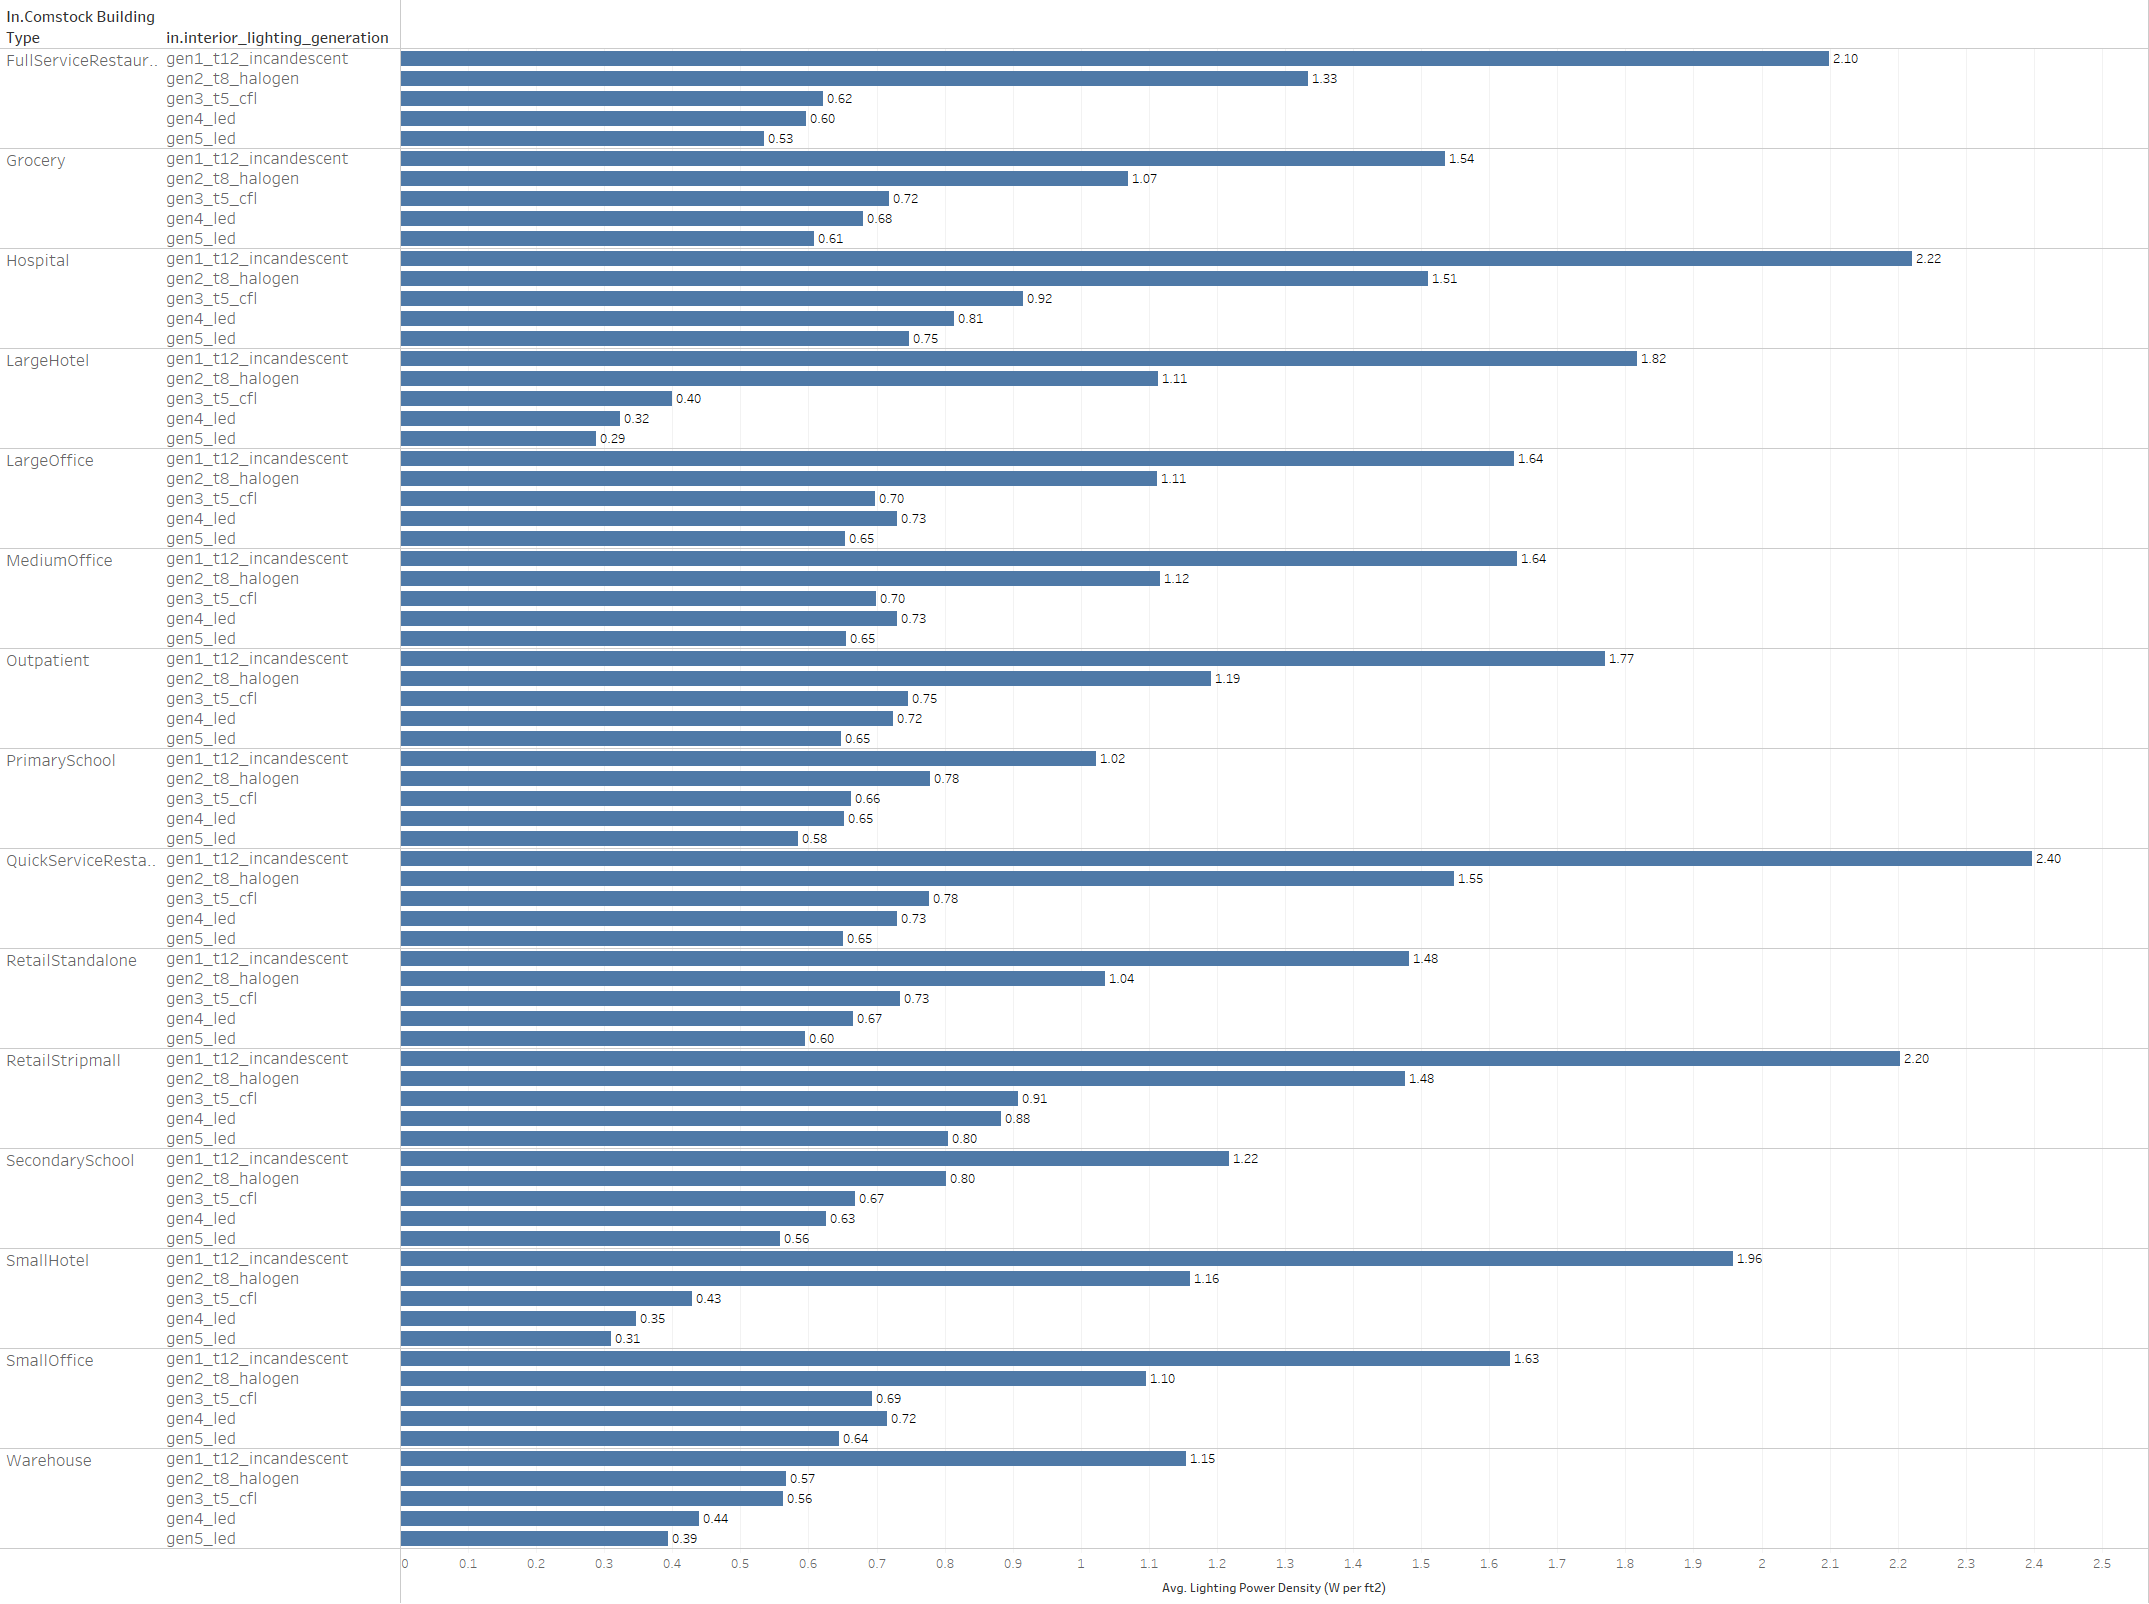
\includegraphics[width=1\textwidth]{figures/interior_lighting_lpd.png}
    \caption[Average interior lighting power density by building type and lighting generation]{Average interior lighting power density by building type and lighting generation.}
    \label{fig:interior_lighting_lpd}
\end{figure}

\pagebreak
\subsubsection{Distribution of Lighting Technologies}

Lighting generations were assigned to each building model during sampling based on the year of, and energy code in force during, the last interior lighting replacement.  Probability distributions were generated first by using an approximate start and end year for when each technology generation was being installed in commercial buildings (Table \ref{tab:ltg_gen_year}). A Gaussian distribution was generated for each lighting generation using these start and end years, and the resulting distribution for each year of last interior lighting replacement was normalized to create 0--1 probabilities. The probability distributions were duplicated for each energy code in force and were further modified to ensure they were realistic (i.e., generation 1 was not installed in a ComStock 90.1-2013 building). This was done using a cutoff generation for each energy code in force (Table \ref{tab:ltg_cutoff_gen}). Each of the lighting generations were also assigned an arbitrary weight to scale the distributions. This was done to represent realistic installation trends. For example, although the installation years of generation 2 (T8s) and generation 3 (T5s) overlapped, generation 2 (T8s) was more popular. T5s were not that much more efficient than T8s compared to the difference between T8s and T12s, and T5s cost more. Furthermore, T5s have different bi-pin geometry compared to T8s and T12s, meaning replacing T8s or T12s with T5s requires changing fixtures in addition to lamp costs. For those reasons, generation 2 (T8s) are a greater portion of the stock than generation 3 (T5s).

\begin{table}
\small
\centering
\caption[Interior Lighting Generation Cutoff by Energy Code]{Interior Lighting Generation Cutoff by Energy Code}
\label{tab:ltg_cutoff_gen}
\begin{tabular}{|l|l|}
\hline
\textbf{Energy Code in Force} & \textbf{Cutoff Generation} \\ \hline
ComStock DOE   Ref Pre-1980     & gen1\_t12\_incandescent      \\ \hline
ComStock DOE   Ref 1980--2004    & gen1\_t12\_incandescent      \\ \hline
ComStock   90.1-2004            & gen1\_t12\_incandescent      \\ \hline
ComStock   90.1-2007            & gen2\_t8\_halogen            \\ \hline
ComStock   90.1-2010            & gen2\_t8\_halogen            \\ \hline
ComStock   90.1-2013            & gen2\_t8\_halogen            \\ \hline
ComStock   90.1-2016            & gen3\_t5\_cfl                \\ \hline
ComStock   90.1-2019            & gen4\_led                    \\ \hline
ComStock DEER   Pre-1975        & gen1\_t12\_incandescent      \\ \hline
ComStock DEER   1985            & gen1\_t12\_incandescent      \\ \hline
ComStock DEER   1996            & gen1\_t12\_incandescent      \\ \hline
ComStock DEER   2003            & gen1\_t12\_incandescent      \\ \hline
ComStock DEER   2007            & gen2\_t8\_halogen            \\ \hline
ComStock DEER   2011            & gen2\_t8\_halogen            \\ \hline
ComStock DEER   2014            & gen3\_t5\_cfl                \\ \hline
ComStock DEER   2015            & gen3\_t5\_cfl                \\ \hline
ComStock DEER   2017            & gen4\_led                    \\ \hline
ComStock DEER   2020            & gen4\_led                    \\ \hline
\end{tabular}
\end{table}

Finally, an additional level of diversity was added to the process.  Small commercial buildings (<50,000 ft$^2$) tend to retrofit their lighting technology less frequently than large commercial buildings (>50,000 ft$^2$) \citep{neea2019cbsa}.  To capture this, we changed the interior lighting lifespan values so that large buildings updated their lighting every seven years on average and small buildings updated their lighting every 13 years. These time spans average to 10 years, which matches the median EUL interior lighting used previously.

The distributions were validated against data from the 2015 Lighting Market Characterization Study \citep{doe2015lmc} and the 2019 Solid State Lighting Report \citep{doe2019ssl}. ComStock sampling results from 2017 and 2020 simulation years were compared against the data from these two studies from the same years, which is referred to as ``truth'' data in this document. The comparison results for 2017 and 2020 simulation years, as well as the data from the two reports for 2015, 2025, 2030, and 2035, are shown in Figure \ref{fig:ltg_compare_dist}.

\begin{figure} [b!]
    \centering 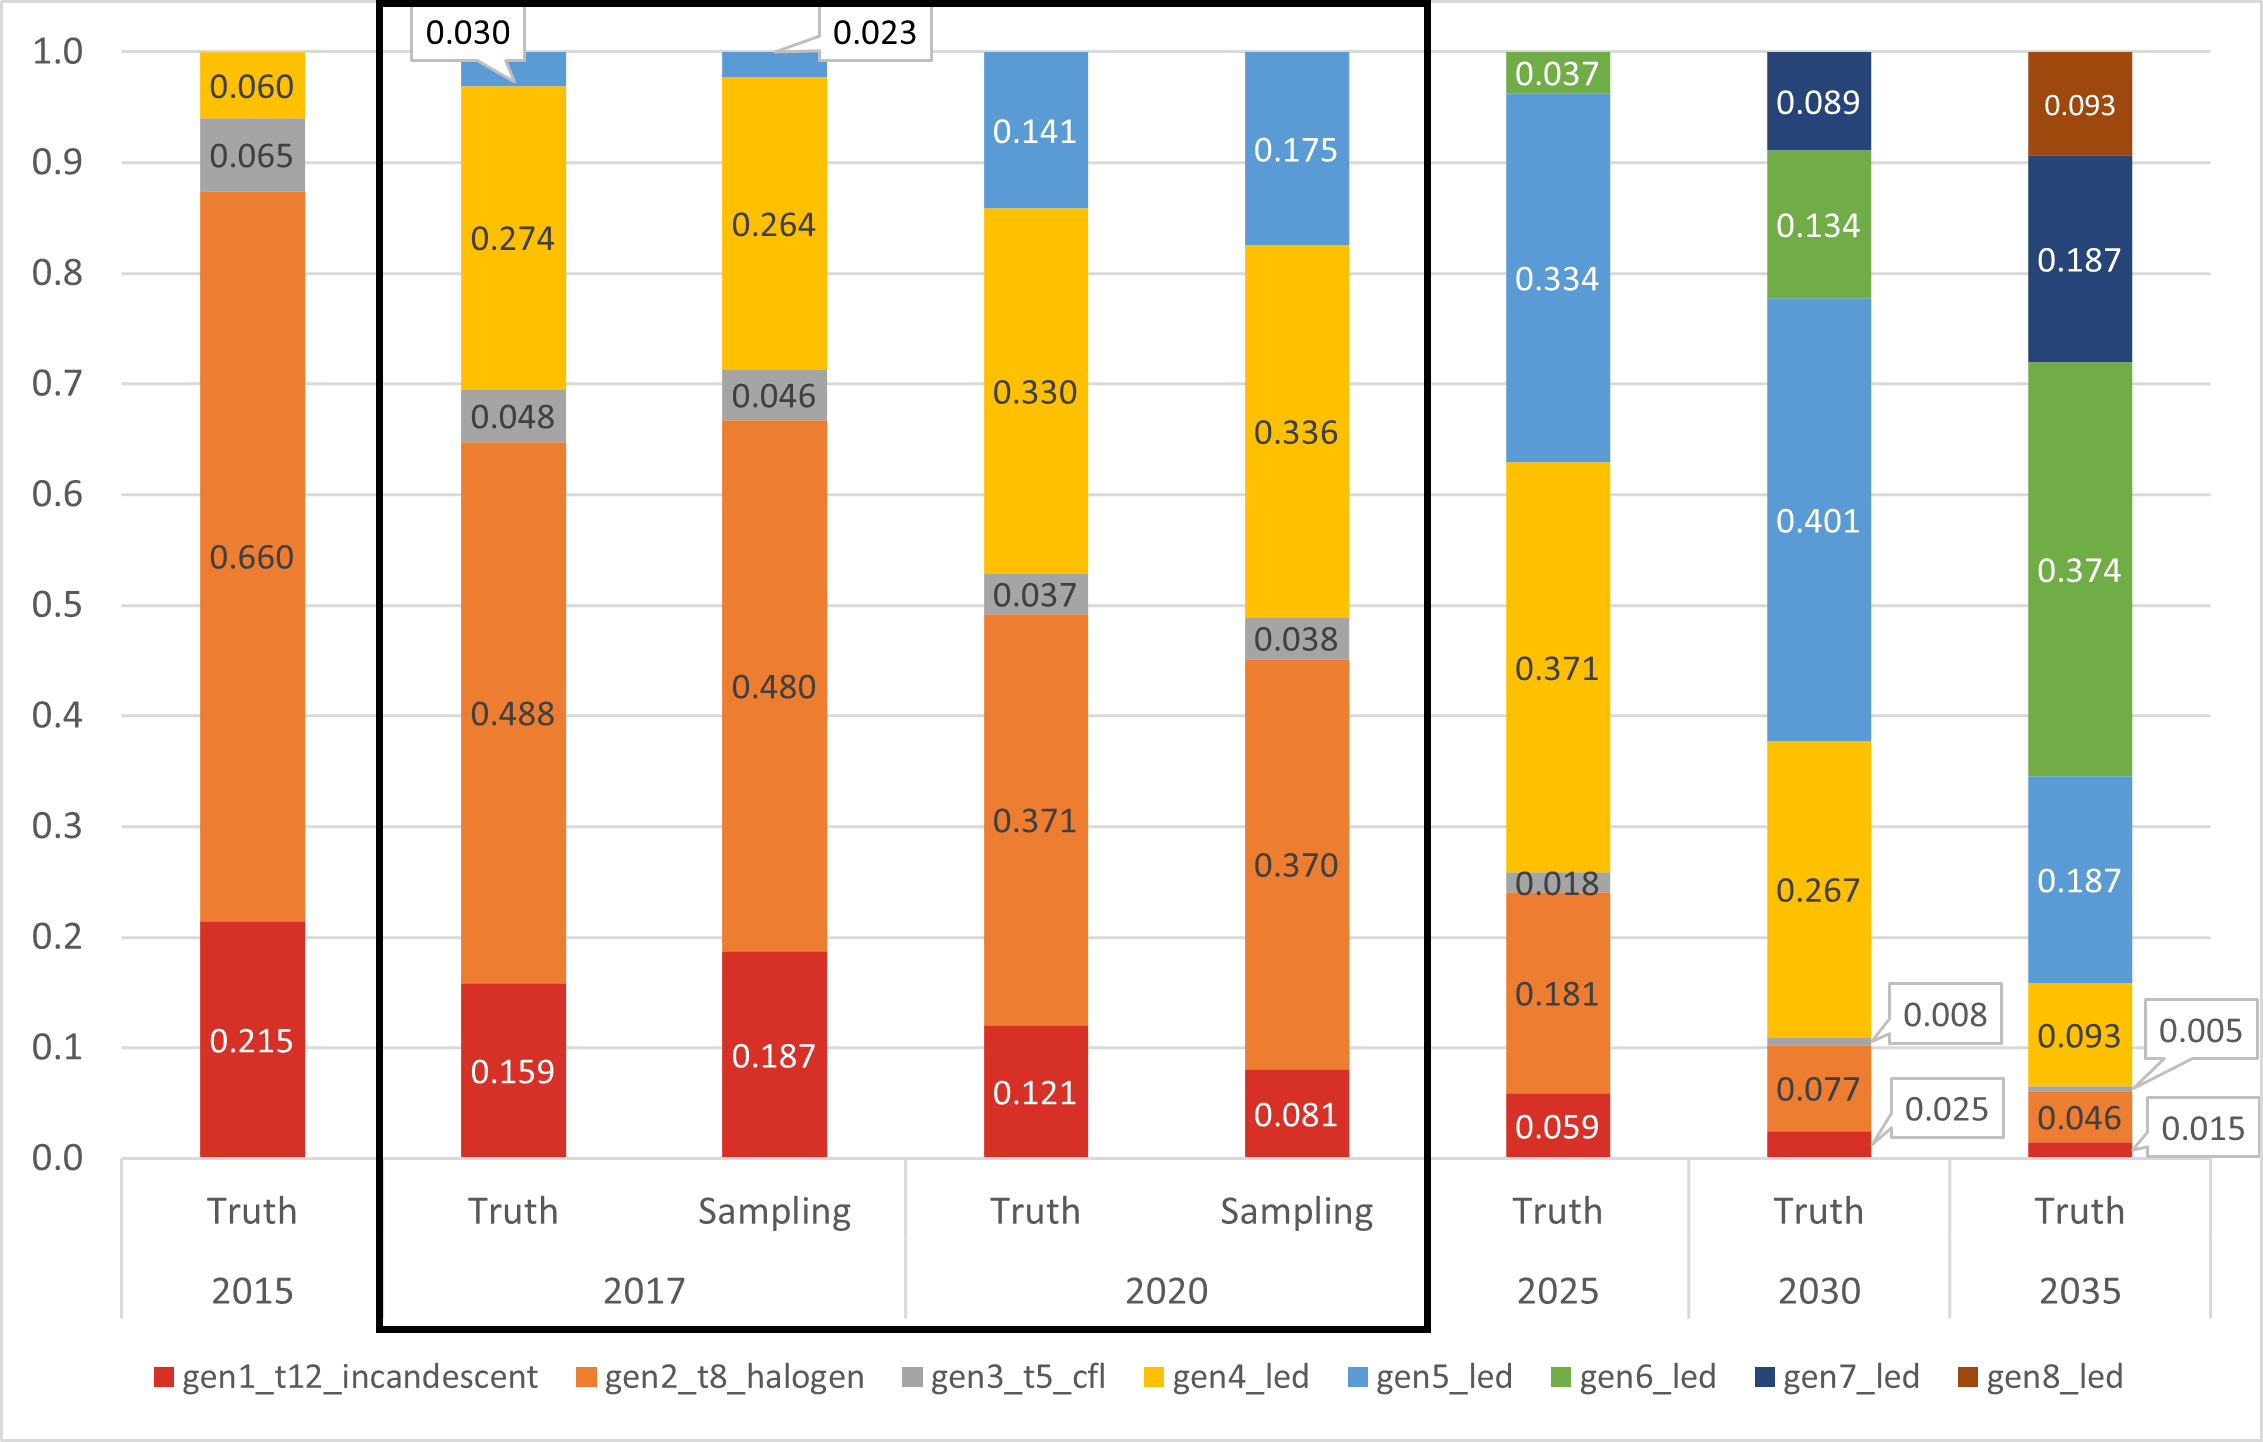
\includegraphics[width=0.8\textwidth]{figures/ltg_truth_vs_sampling.png}
    \caption[Interior lighting generation distributions]{``Truth'' lighting generation distribution data from \cite{doe2015lmc} and \cite{doe2019ssl}, and comparison of 2017 and 2020 ComStock sampling results.}
    \label{fig:ltg_compare_dist}
\end{figure}

Simulation years 2017 and 2020 were the focus of validation because they represent the range of simulation years typically run for ComStock. Additionally, for a given iteration of the lighting generation distributions, the comparison results were inconsistent across simulation years. For example, for a set of lighting generation distributions that showed close comparisons for 2017 and 2020, years 2025--2035 were significantly different compared to the other future projections.  With improvements to the script that produces the distributions, close comparisons across all simulation years should be feasible.

Table \ref{tab:ltg_gen_tsv} provides a snapshot of the final probability distributions, which show a gradual shift to higher generations as the year of the last interior lighting replacement increases. For this code year (ComStock 90.1-2013), generation 1 lighting technologies would likely not be installed. This is reflected in the distributions, as the minimum lighting generation installed is at least generation 2.  The relative popularity of each generation is also apparent in the distributions: generation 2 has a much higher probability of being installed in any year than generation 3, a less popular technology set.

\pagebreak

There are two primary areas for improvement for this process:
\begin{itemize}
\item The first is in the initial Gaussian distributions. Although there is good data about when the lighting generations were first installed and when they finally lost popularity, information about when the generations peaked in their install popularity is not available. The current method assumes that the peak is at the midpoint of the start and end year. This is most likely incorrect. If data on the peak year of each generation could be collected, this would improve the distribution generation process.
\item The second improvement area is the final weighting process. The weights are currently determined using a guess-and-check method.  Further improvements to the distribution script would make this method more robust (e.g., using an optimization algorithm).
\end{itemize}

Figure \ref{fig:ltg_size_dist} shows the breakdown of lighting generation distribution (by count) by building size for 2018, the year the current ComStock data set represents the United States building stock. Small buildings are under 50,000 ft$^2$ and are assumed to have slower retrofit frequency than larger buildings (>50,000 ft$^2$). The data trend matches this assumption, as there is a larger percentage of smaller building models that have generation 1 and 2 lighting technologies.

Figure \ref{fig:ltg_btype_dist} provides a breakdown of lighting generation distributions by building type. There is not huge variation among the building types. However, building types that are typically smaller (quick service restaurants, small offices, strip malls) lag behind the other building types in terms of lighting technology.  This is consistent with the data in Figure \ref{fig:ltg_size_dist}.

\begin{figure}[ht!]
    \centering 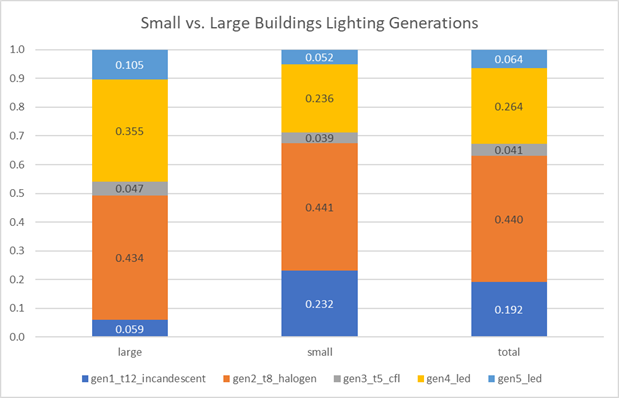
\includegraphics[width=0.8\textwidth]{figures/ltg_size_dist.png}
    \caption[Fraction of installed lighting generations by building size] {Fraction of installed lighting generations by building size (count-based distribution).}
    \label{fig:ltg_size_dist}
\end{figure}

\begin{figure}[ht!]
    \centering 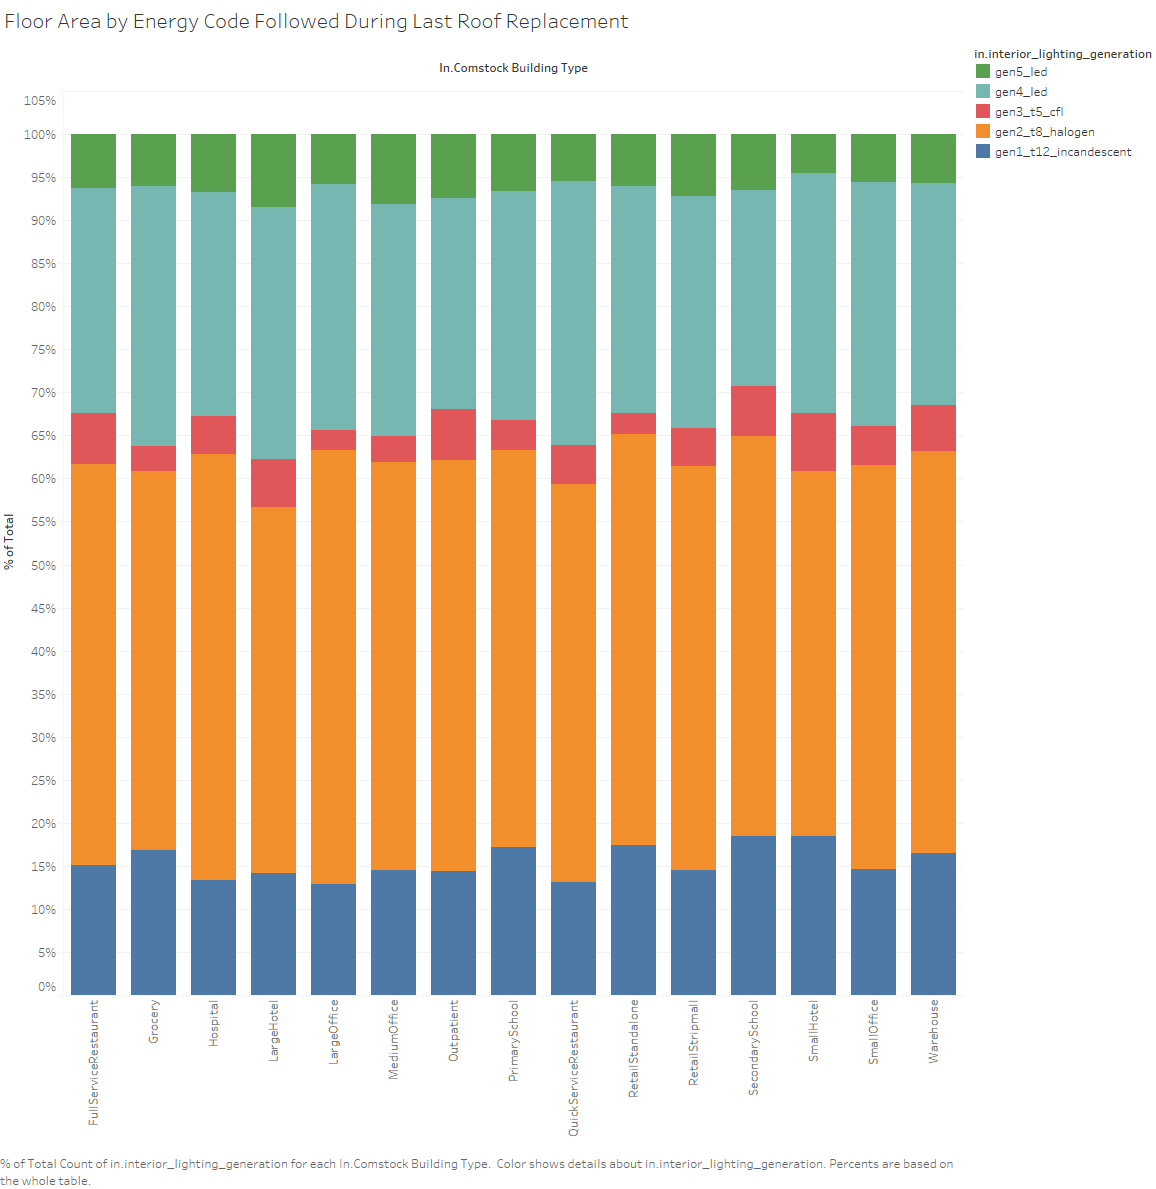
\includegraphics[width=0.9\textwidth]{figures/ltg_btype_dist.png}
    \caption[Fraction of installed lighting generation by building type]{Fraction of installed lighting generation by building type (count-based distribution).}
    \label{fig:ltg_btype_dist}
\end{figure}

\pagebreak

\subsubsection{Default Interior Lighting Schedules}
Default interior lighting schedules come from the openstudio-standards DOE prototype building models \citep{deru_2011}.  The End-Use Load Profiles project derived new default lighting schedules for restaurant, retail, education, office, and warehouse buildings, detailed in Section 3.3.1 of the EULP report: ``Interior Lighting Schedules'' \citep{eulp_method_2022}. A full list of default ComStock schedules is available as a  \href{https://github.com/NREL/openstudio-standards/blob/master/lib/openstudio-standards/standards/ashrae_90_1/ashrae_90_1_2013/comstock_ashrae_90_1_2013/data/ashrae_90_1.schedules.json}{schedules .json file} on the openstudio-standards GitHub repository.

Additional changes to default schedules include:

\begin{itemize}
  \item The peak lighting value in the end-use data derived hourly schedule for office spaces is now 0.85 instead of the original ~0.5.
  \item Quick service restaurants and kitchens use the FoodService\_Restaurant BLDG\_LIGHT\_EndUseData schedule rather than the prototype schedule.
  \item All large hotel guest room lighting schedules use HotelLarge BLDG\_LIGHT\_GUESTROOM\_SCH\_2013.
  \item All small hotel guest rooms follow the same default lighting schedule, with the midday lighting fraction changed from the prototype schedule value of ~0.3 to 0.15. Vacant guest rooms use an always off lighting schedule.
\end{itemize}

Interior lighting schedules are adjusted to correspond with the building's operating hours, as described in Section \ref{sec:hoo}.

\subsubsection{Interior Lighting Schedule Magnitude Variability}
Section 3.3.4 in the End-Use Load Profiles project report, ``Interior Lighting Schedule Magnitude Variability'' \citep{eulp_method_2022}, details the derivation of base-to-peak values applied to the default lighting schedules.

Figure \ref{fig:ltg_bpr} shows the distribution of base-to-peak ratios (BPRs) in the stock by building type for weekdays and weekends.  Note that this methodology was not applied to hospital, outpatient, small and large hotel, and warehouse building types, due to a lack of data.

\begin{figure}
    \centering 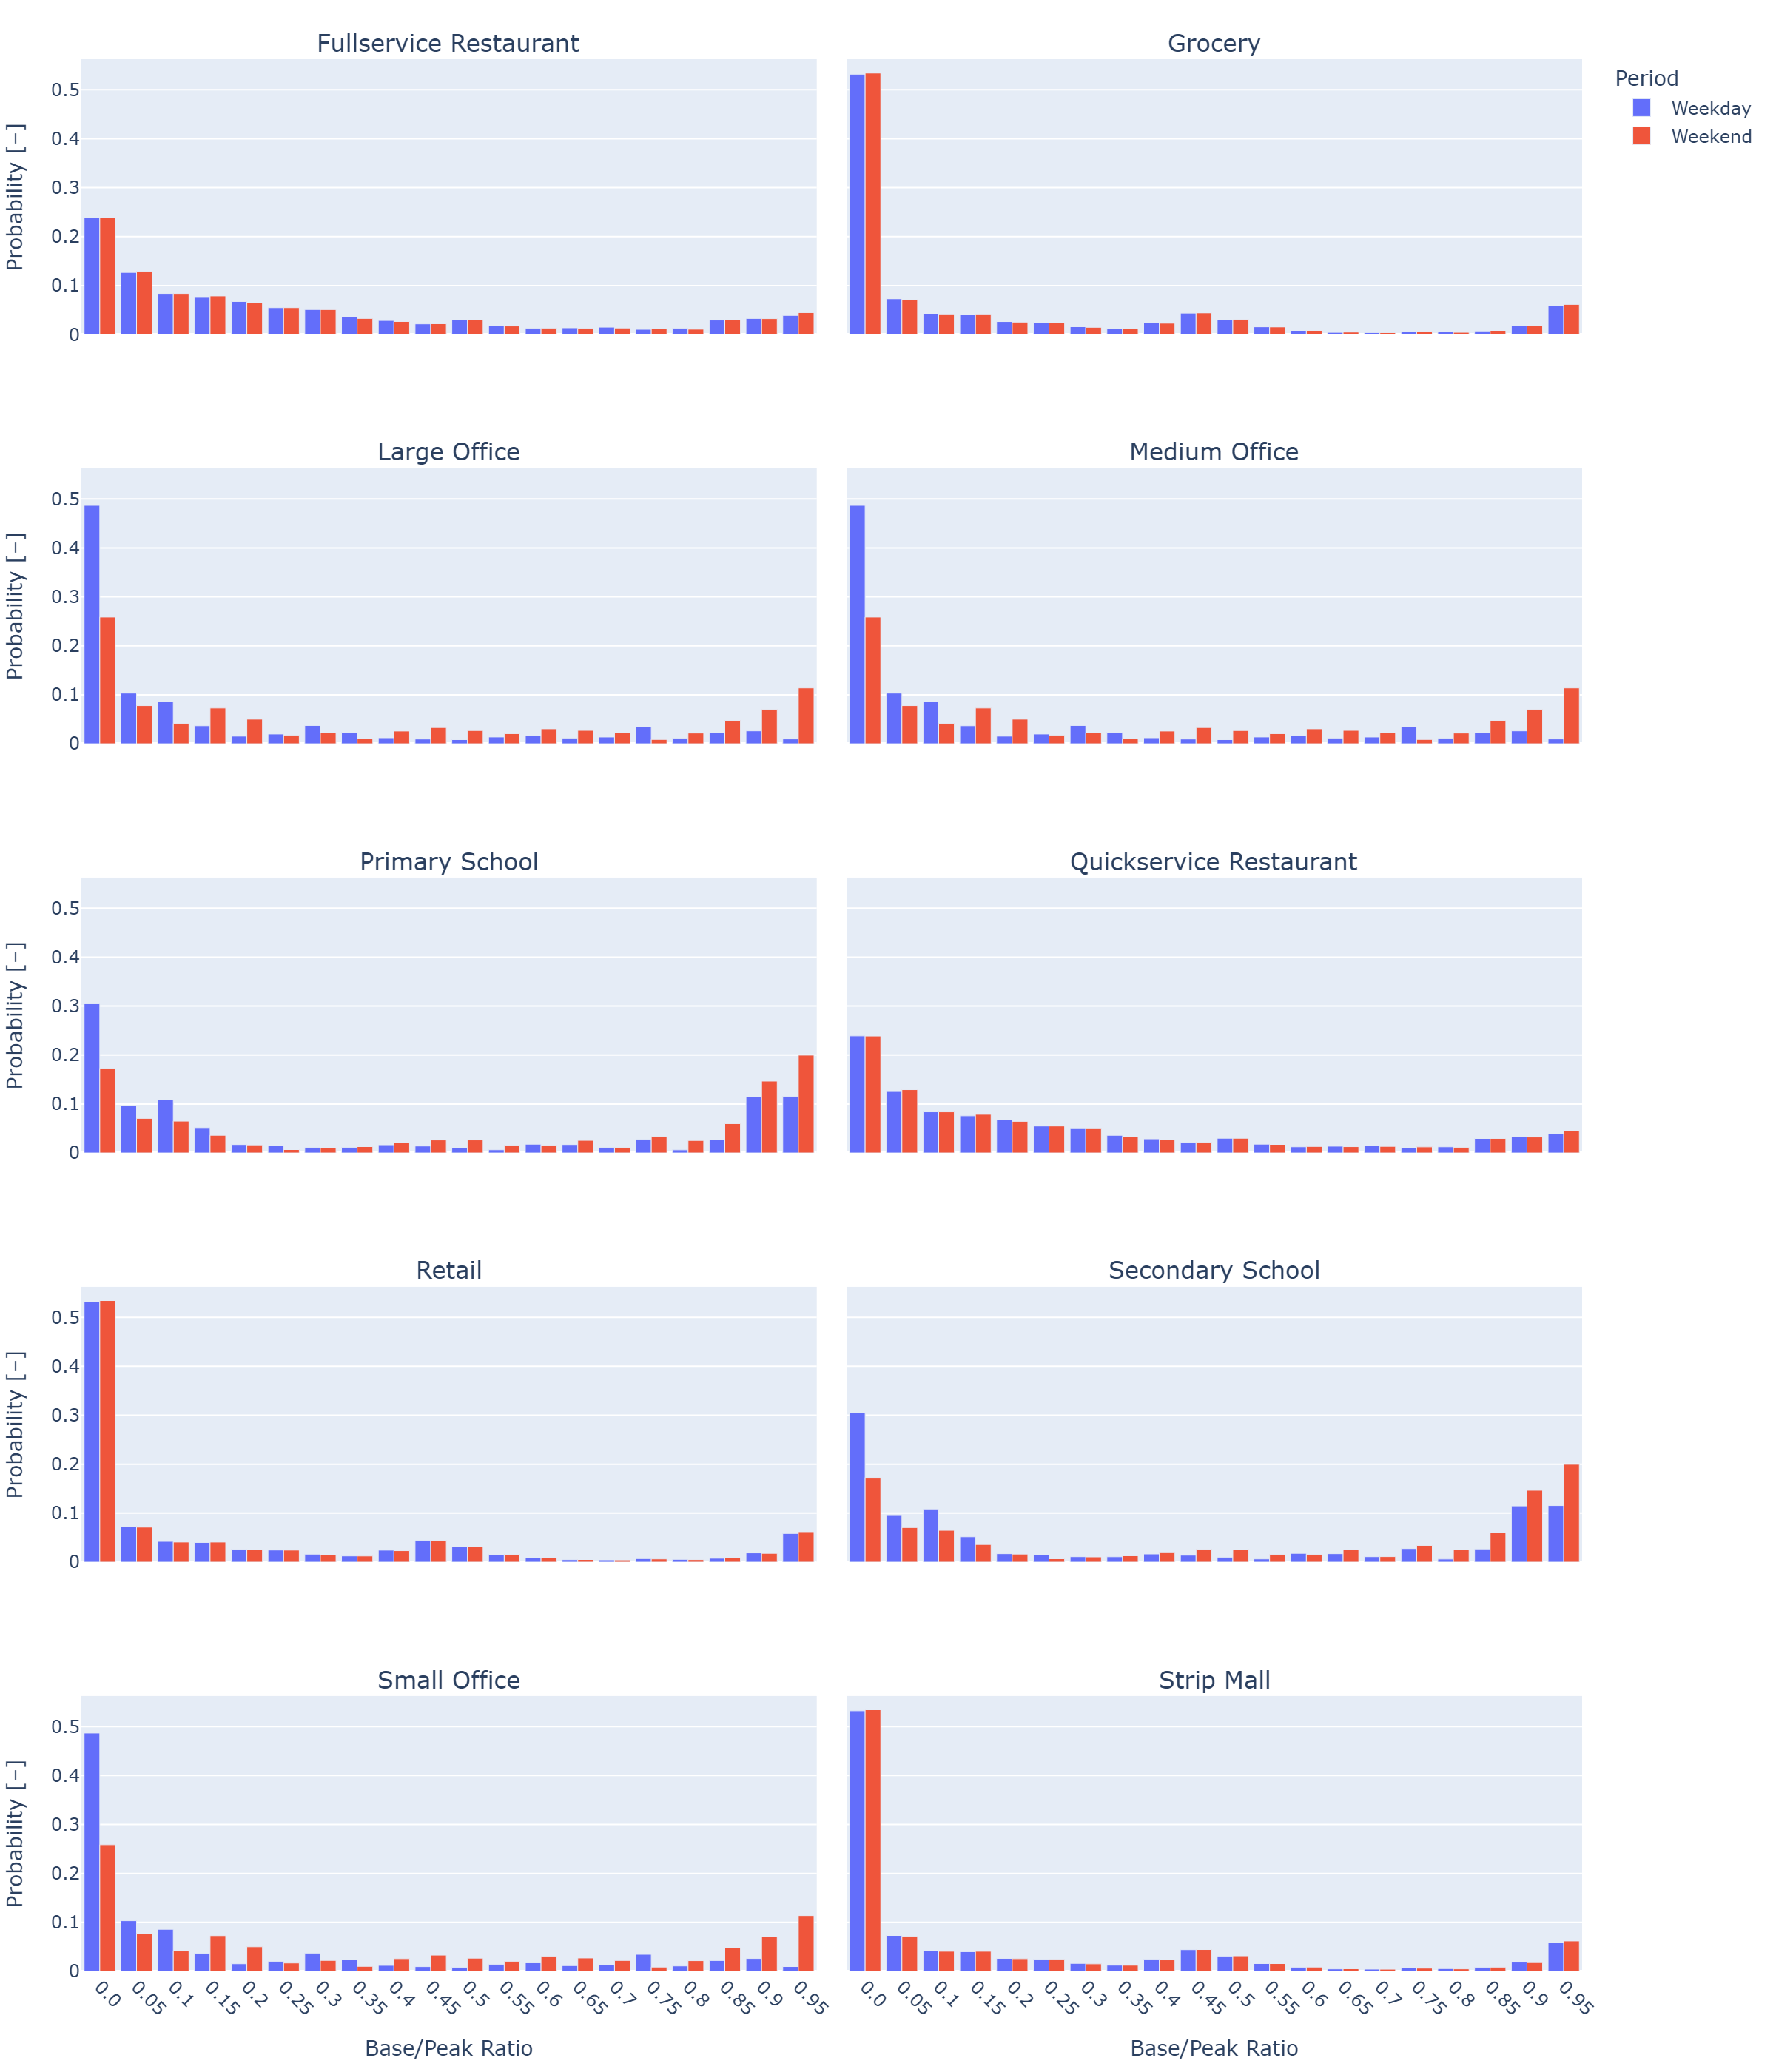
\includegraphics[width=0.9\textwidth]{figures/ltg_sch_bpr.png}
    \caption[Weekday and weekend lighting base-to-peak ratios by building type]{Weekday and weekend lighting base-to-peak ratios by building type. Base-to-peak ratio is on the x-axis, and fraction of the stock is on the y-axis.}
    \label{fig:ltg_bpr}
\end{figure}

\begin{figure}
    \centering 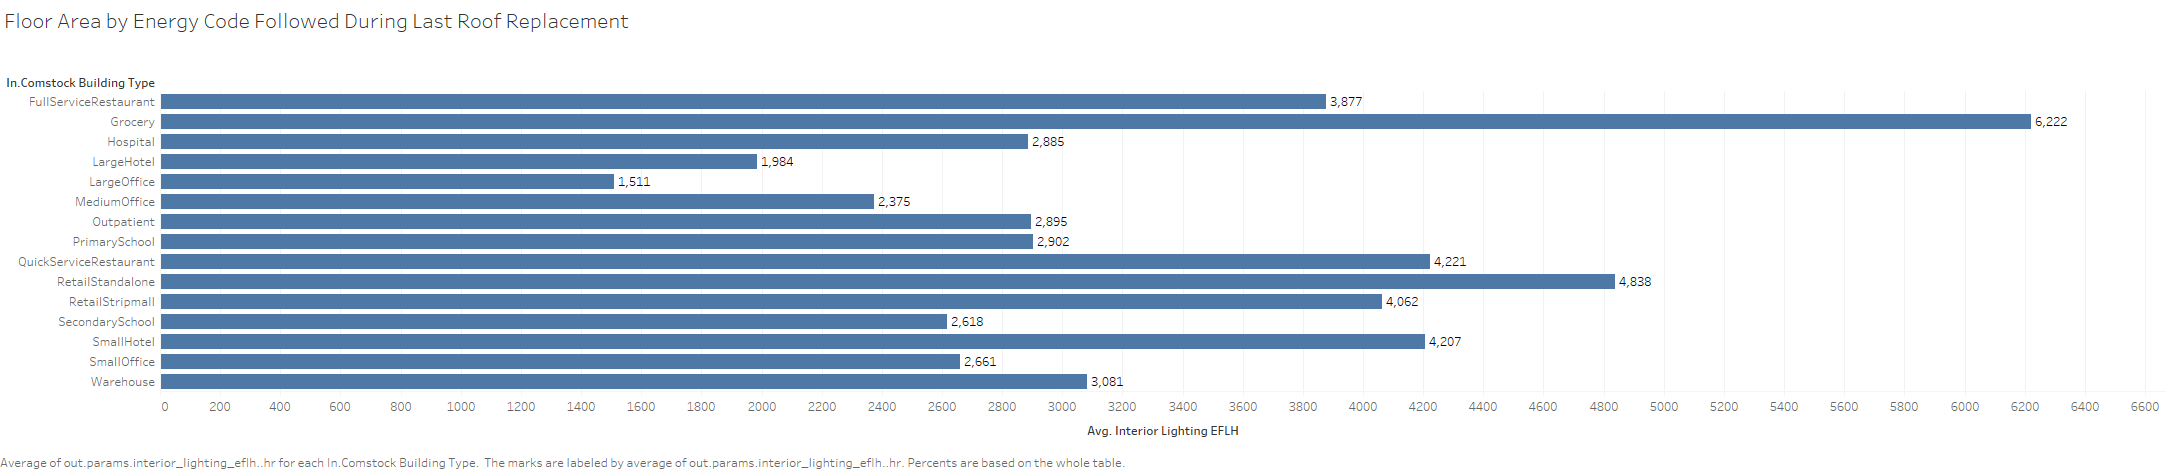
\includegraphics[width=1.0\textwidth]{figures/interior_lighting_eflh.png}
    \caption[Average interior lighting equivalent full load hours by building type]{Average interior lighting equivalent full load hours by building type.}
    \label{fig:interior_lighting_eflh}
\end{figure}

\subsection{Exterior Lighting}
Exterior lighting is all outdoor lighting at the building site, including lighting for parking, walkways, doorways, canopies, building facades, signage, and landscaping.

\subsubsection{Parking Area Lighting}
Parking area lighting accounts for the majority of exterior lighting in the stock \citep{doe2015lmc}. Parking lighting is calculated as the parking area times the installed lighting power per unit of parking area. Parking area is based on the estimated number of parking spots per student for schools, per unit for hotels, per bed for hospitals, and per building floor area for all other building types.  Parking spots are assumed to be 405 ft$^2$. Table \ref{tab:parking} details these assumptions.

Lighting power for a given parking area is determined from the 2015 U.S. Lighting Market Characterization report, which assumes an average of 216 Watts (W) per parking lighting system, or 0.0410 W/ft\textsuperscript{2} (per equation \ref{ext_light_eqn}). Base parking lighting power allowance values for each vintage were reduced by a calculated factor such that the building-count weighted parking lighting power density came out to the 0.0410 W/ft\textsuperscript{2} target.  Note that this calculation is from 2015, so it overestimates the amount of exterior lighting in the stock, which has been changing over to use LEDs. The values for each vintage are shown in Table~\ref{tab:exterior_lighting_power}.

\begin{align}
\label{ext_light_eqn}
LPD = \left(\frac{216\,W}{\text{lighting system}}\right) \cdot \left(\frac{1\,\text{lighting system}}{13\,\text{parking spots}}\right) \cdot \left(\frac{1\,\text{parking spot}}{405\,\text{ft}^2}\right) = 0.0410\,W/\text{ft}^2
\end{align}


\subsubsection{Other Exterior Lighting}
Non-parking exterior lighting is determined by the exterior lighting allowance specified in ASHRAE 90.1 for exterior lighting zone 3 (All Other Areas). Length and area estimates are determined from the values in Table \ref{tab:entryways}. The building facade area is calculated from the model as the ground floor exterior wall area. The lighting power allowance is matched to the 90.1 code for each vintage. The exterior lighting power allowances are shown in Table~\ref{tab:exterior_lighting_power}. Note that although 90.1 includes exterior lighting, the only forms of exterior lighting included in ComStock are parking areas, building facades, main entry doors, other doors, drive through windows, entry canopies, and emergency canopies. Notably, ComStock does not include lighting for exterior signage.
